\documentclass[12pt,a4paper]{article}
\usepackage[utf8]{inputenc}
\usepackage[T1]{fontenc}
\usepackage{amsmath}
\usepackage{amsfonts}
\usepackage{amssymb}
\usepackage{graphicx}
\usepackage{geometry}
\usepackage{mathtools}
%\usepackage{diagrams}
\usepackage[document]{ragged2e}
\usepackage{wasysym}
\usepackage{pgfplots}
\usepackage{ mathrsfs }
\usepackage{braket}
\usepackage{simpler-wick}
\usepackage{tikz}
\usetikzlibrary{decorations.markings}
\usepackage{tikz-feynman}
\usepackage{subcaption}
\usepackage{bm}
\usepackage{slashed}
\usepackage{tensor}
\usepackage{hyperref}
\usepackage{float}
\usetikzlibrary{calc}
\tikzset{
	myarrow/.style={stealth-,shorten >=3pt,shorten <=3pt}
}
\pgfplotsset{
	lineplot/.style={
		black,
		dashed,
		very thin,
		samples y=0
	},
	coordinate line/.style={
		black,
		samples y=0
	},
	point/.style={
		only marks,
		mark=*,
		black,
		mark size=0.5pt
	}
}
\title{Topics in Mathematical Physics}
\author{Ben Karsberg}
\date{2021-22}
\newgeometry{vmargin={15mm}, hmargin={20mm,20mm}}
\numberwithin{equation}{section}
\DeclareMathSymbol{:}{\mathord}{operators}{"3A}
\begin{document}
	\maketitle
	\section{Preface}
	\begin{itemize}
		\item These notes were written up for the postgraduate masters course in mathematical physics at the University of Edinburgh
		\item The topic this year was 'Applications of Geometry in Physics'
		\item It was lectured by James Lucietti, who's notes are unfortunately only available on the Edinburgh intranet
		\item These notes were largely produced with those official notes as reference
		\item These notes were written primarily with myself in mind; it has some colloquialisms in it, and some topics are presented in the way I best understand them, and not necessarily the `best' way
		\item The notes are also exclusively bullet pointed because I find prose difficult to digest
		\item Any errors are most certainly mine and not James's - let me know at \href{mailto:benkarsberg@gmail.com}{benkarsberg@gmail.com} if you note any bad ones
		\item Generally, text in \textit{italic} is the definition of something the first time it shows up, and text in \textbf{bold} is something I think is important/want to remember/found tricky when writing these up
		\item Summation convention is implicit throughout this entire set of notes, unless explicitly stated otherwise
		\item Euclidean spatial vectors are denoted by e.g. $\mathbf{v}$, and 4-vectors are denoted by just $v=(v^{0},\mathbf{v})$
		\item The metric signature is $\eta_{\mu\nu}=\text{diag}(+1,-1,-1,-1)$ unless stated otherwise
		\item $\hbar=c=1$
		\item I hope these notes are helpful to someone who isn't me - enjoy!
	\end{itemize}
	\newpage
	\section{Differential Geometry Preliminaries}
	\begin{itemize}
		\item This course is all about geometry, almost entirely differential
		\item Differentiable geometry is a listed prerequisite for this course, but I haven't done any properly, with the exception of pseudo-Riemannian geometry in coordinate bases in a GR course last year
		\item Therefore, we need to set the scene
		\item The principal arena for differential geometry is a \textbf{differential manifold}:
		\begin{itemize}
			\item Informally, this is a set $M$ that locally looks like $\mathbb{R}^{n}$
			\item Formally, this is a topological space $M$ equipped with a collection of charts $\{(U_{\alpha},\phi_{\alpha})\}$ called an \textbf{atlas}, where $\{U_{\alpha}\}$ is an open cover of $M$ and $\phi_{\alpha}\;:\;U_{\alpha}\to V_{\alpha}\subset\mathbb{R}^{n}$ are homeomorphisms
		\end{itemize}
		\item The image we want in mind is something like this, generalised to $\mathbb{R}^{n}$ rather than just $\mathbb{R}^{2}$:
		\begin{figure}[H]
			\centering
		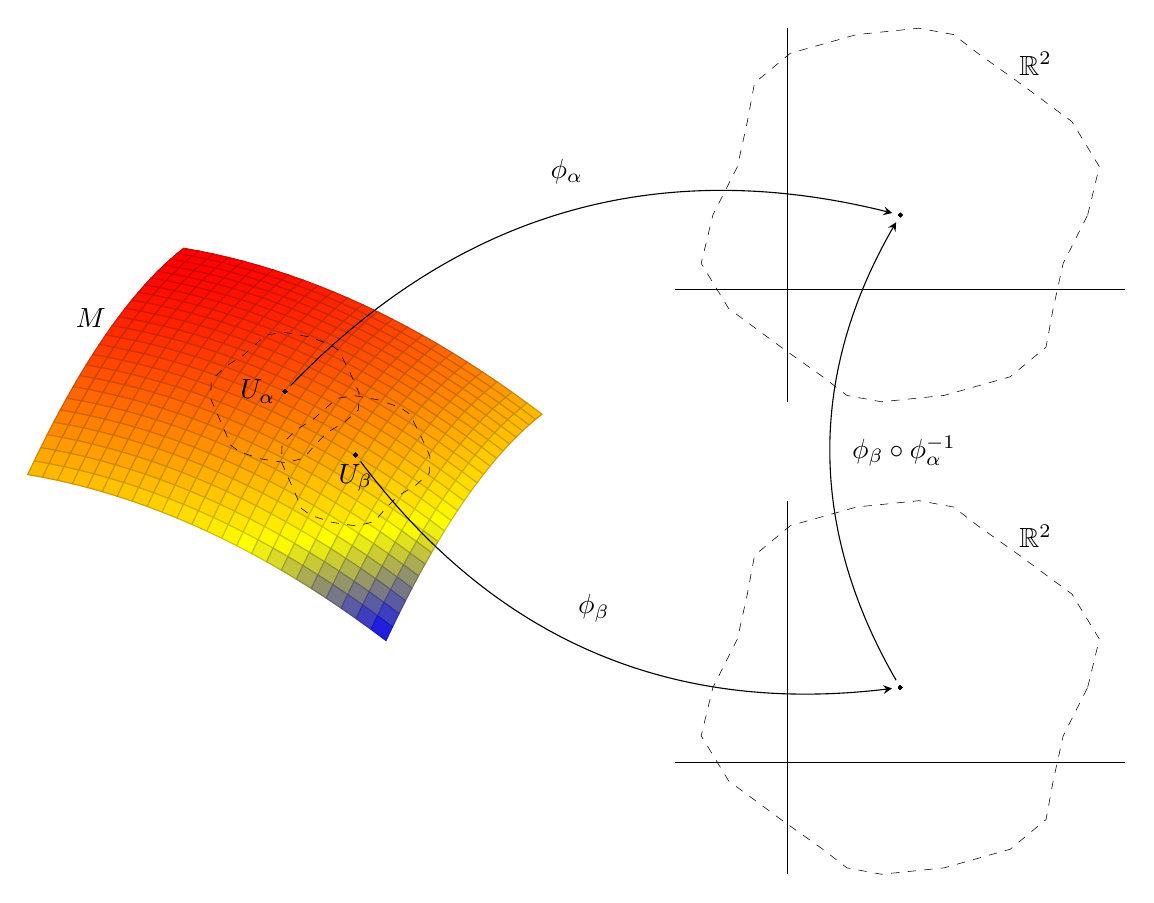
\begin{tikzpicture}
			\begin{axis}[
				name=mfd,
				axis lines=none,
				declare function={
					f(\x,\y)=10-(\x^2+\y^2);
				},
				declare function={
					c_x(\t)=(cos(\t)+(sin(5*\t)/10))/3+1;
				},
				declare function={
					c_y(\t)=(sin(\t))/2-1;
				},
				declare function={
					c_z(\t)=f(c_x(\t),c_y(\t));
				},
				declare function={
					x_0(\t)=-1.2;
				},
				declare function={
					x_1(\t)=0.8;
				}
				]
				\addplot3[surf,domain=0:2,domain y=-2:0,]{f(x,y)};
				\addplot3[lineplot,variable=t,domain=0:360] ({c_x(t)},{c_y(t)},{c_z(t)});
				\addplot3[lineplot,variable=t,domain=0:360] ({c_x(t)+0.7},{c_y(t)-0.7},{c_z(t)});
				%\addplot3[coordinate line,variable=t,domain=0:2] (t,{x_0(t)},{f(t,{x_0(t)})});
				%\addplot3[coordinate line,variable=t,domain=-2:0] ({x_1(t)},t,{f({x_1(t)},t)});
				\addplot3[point] (1,-1,{f(1,-1)}) coordinate (a);
				\addplot3[point] (1.7,-1.7,{f(1,-1)}) coordinate (c);
				%\addplot3[point](.5,{x_0(.5)},{f(.5,{x_0(.5)})}) coordinate (x_dot);
				%\addplot3[point]({x_1(-.5)},-.5,{f({x_1(-.5)},-.5)}) coordinate (y_dot);
			\end{axis}
				\draw (a) node [left] {$U_{\alpha}$};
				\draw (c) node [below] {$U_{\beta}$};
			\begin{axis}[
				at={($(mfd.north east)+(1cm,3cm)$)},
				anchor=north west,
				axis lines=none,
				declare function={
					c_x(\t)=(cos(\t)+(sin(5*\t)/10))/3+1;
				},
				declare function={
					c_y(\t)=(sin(\t))/2-1;
				},
				declare function={
					x_0(\t)=-1.2;
				},
				declare function={
					x_1(\t)=0.8;
				}
				]
				\addplot[lineplot,variable=t,domain=0:360]({c_x(t)},{c_y(t)});
				\addplot[point] (1,-1) coordinate (b);
				\addplot[coordinate line,variable=t,domain=0.6:1.4](t,{x_0(t)});
				\addplot[coordinate line,variable=t,domain=-1.5:-0.5]({x_1(t)},t);
				%\addplot[point](.8,-.5) coordinate (P1);
				%\addplot[point](.6,-1.2) coordinate (P2);
			\end{axis}
			\draw [myarrow] (b) to[bend right] node [above=7pt] {$\phi_{\alpha}$} (a);
			\draw (13,7.5) node [above] {$\mathbb{R}^{2}$};
			\draw (13,1.5) node [above] {$\mathbb{R}^{2}$};
			\draw (1,4.3) node [above] {$M$};
			%\draw [myarrow] (P1) to[bend left] ++(-1cm,1cm) node[above] {$(x \circ \gamma_{(1)})$};
			%\draw [myarrow] (P2) to[bend left] ++(-3cm,-1cm) node[above] {$(x \circ \gamma_{(0)})$};
			\begin{axis}[
				at={($(mfd.north east)+(1cm,-3cm)$)},
				anchor=north west,
				axis lines=none,
				declare function={
					c_x(\t)=(cos(\t)+(sin(5*\t)/10))/3+1;
				},
				declare function={
					c_y(\t)=(sin(\t))/2-1;
				},
				declare function={
					x_0(\t)=-1.2;
				},
				declare function={
					x_1(\t)=0.8;
				}
				]
				\addplot[lineplot,variable=t,domain=0:360]({c_x(t)},{c_y(t)});
				\addplot[point] (1,-1) coordinate (d);
				\addplot[coordinate line,variable=t,domain=0.6:1.4](t,{x_0(t)});
				\addplot[coordinate line,variable=t,domain=-1.5:-0.5]({x_1(t)},t);
			\end{axis}
			\draw [myarrow] (d) to[bend left] node [above=7pt] {$\phi_{\beta}$} (c);
			\draw [myarrow] (b) to[bend right] node [right=4pt] {$\phi_{\beta}\circ\phi_{\alpha}^{-1}$} (d);
		\end{tikzpicture}
		\end{figure}
		\item Essentially, a chart $(U,\phi)$ assigns coordinates to a point $p\in U$ given by $\phi(p)=(x^{1}(p),\ldots,x^{n}(p))$, usually written $\phi=\left(x^{i}\right)$
		\item Importantly, the \textbf{transition functions} $\phi_{\beta}\circ\phi_{\alpha}^{-1}\;:\;\phi_{\beta}(U_{\alpha}\cap U_{\beta})\to\phi_{\alpha}(U_{\alpha}\cap U_{\beta})$ should be $C^{\infty}(\mathbb{R}^{n})$ bijections between open subsets of $\mathbb{R}^{n}$ (see diagram)
		\item Essentially, all changes of coordinates are given by a smooth map
		\item The atlas allows us to define calculus on a manifold, and we can classify a hierarchy of objects on $M$:
		\begin{itemize}
			\item $C^{\infty}(M)$ is the set of all smooth functions on $M$, with the function of a standard commutative algebra
			\item The \textbf{tangent space} $T_{p}M$ at $p\in M$ is the $n$-dimensional vector space of directional derivatives at $p$; that is, the space of all $\mathbb{R}$-linear maps $X_{p}\;:\; C^{\infty}(M)\to\mathbb{R}$ obeying the Leibnitz/product rule
			\begin{equation}
				X_{p}(fg)=X_{p}(f)g(p)+f(p)X_{p}(g)
			\end{equation}
			for all $f,g\in C^{\infty}(M)$
			\item The elements $X_{p}\in T_{p}M$ are called \textbf{tangent vectors}; if we consider a smooth curve $\gamma\;:\;(a,a)\to M$ where $\gamma(0)=p$, we can define a tangent vector to the curve called the velocity $\dot{\gamma}\in T_{p}M$ by $\dot{\gamma}(f)=\left.\frac{d}{dt}f(\gamma(t))\right|_{t=0}$, and all tangent vectors arise like this
			\item A \textbf{vector field} $X\in\mathfrak{X}(M)$ is a smooth assignment to each $p\in M$ of a tangent vector $X_{p}\in T_{p}M$ (or more formally, a section of the \textbf{tangent bundle} $TM$)
			\item A \textbf{differential} $k$\textbf{-form} $\alpha_{p}$ at $p\in M$ is a smooth alternating multilinear map $\alpha_{p}\;:\;T_{p}M\times\ldots\times T_{p}M\to \mathbb{R}$
			\item The set of all $k$-forms is denoted $\Omega^{k}(M)$, where $\alpha(X_{1},\ldots,X_{k})\in C^{\infty}(M)$ and $X_{i}\in\mathfrak{X}(M)$
			\item In particular, 1-forms at $p$ are just dual vectors $\alpha_{p}\in T_{p}^{*}M$
			\item The \textbf{wedge produce} of $\alpha\in\Omega^{k}(M)$ and $\beta\in\Omega^{l}(M)$ is $\alpha\wedge\beta\in\Omega^{k+l}(M)$ where $\alpha\wedge\beta=(-1)^{kl}\beta\wedge\alpha$; in particular, for 1-forms we have
			\begin{equation}
				(\alpha\wedge\beta)(X,Y)=\alpha(X)\beta(Y)-\beta(X)\alpha(Y)
			\end{equation}
			\item The \textbf{exterior derivative} is a $\mathbb{R}$-linear map $d\;:\;\Omega^{k}(M)\to\Omega^{k+1}(M)$ satisfying $d^{2}=0$ and $d(\alpha\wedge\beta=(d\alpha)\wedge\beta +(-1)^{k}\alpha\wedge(d\beta)$
			\item The \textbf{interior derivative} $\iota_{X}\;:\;\Omega^{k}(M)\to\Omega^{k-1}(M)$ is defined by $\iota_{X}\alpha=\alpha(X,\ldots)$ for $X\in\mathfrak{X}(M)$
			\item In particular, if we regard a smooth function $f$ on $M$ as a 0-form, $(df)(X)=X(f)$
			\item \textbf{Tensors} and \textbf{tensor fields} of type $(r,s)$ are very similar to vectors and vector fields, acting as multilinear maps $T\;:\; T_{p}^{*}M\times\ldots T_{p}^{*}M\times T_{p}M\times\ldots T_{p}M\to\mathbb{R}$
			\item The derivative of a smooth map $\phi\;:\;M\to N$ is called the \textbf{push-forward map} $\phi_{*}\;:\;T_{p}M\to T_{\phi(p)}N$ given by
			\begin{equation}
				(\phi_{*}X_{p})(f)=X_{p}(f\circ\phi)
			\end{equation} 
			where $f\in C^{\infty}(N)$
			\item Similarly, the \textbf{pull-back} is $\phi^{*}\;:\;T_{\phi(p)}^{*}N\to T_{p}^{*}M$ given by
			\begin{equation}
				(\phi^{*}\alpha_{\phi(p)})(X_{p})=\alpha_{\phi(p)}(\phi_{*}X_{p})
			\end{equation}
			\item A smooth bijection $\phi\;:\;M\to N$ is called a \textbf{diffeomorphism}, and for a diffeomorphism we have $(\phi^{-1})_{*}=\phi^{*}$
			\item The \textbf{flow} of a vector field $X$ is a 1-parameter group of diffeomorphisms; i.e. a family $\phi_{t}\;:\;M\to M$ such that $\phi_{t+s}=\phi_{t}\circ\phi_{s}$ for all real $t,s$
			\item In particular, the integral curve of $X$ through $p\in M$ is given by $\phi_{t}(p)$ so $X_{p}(f)=\frac{d}{dt}f(\phi_{t}(p))|_{t=0}$
			\item The \textbf{Lie derivative} of a tensor field $T$ along a vector field $X$ is
			\begin{equation}
				\mathcal{L}_{X}T=\left.\frac{d}{dt}(\phi_{t}^{*}T)\right|_{t=0}
			\end{equation}
			where $\phi_{t}$ is the flow of $X\in\mathfrak{X}(M)$
			\item In particular, we have $\mathcal{L}_{X}f=X(f)$ for $f\in C^{\infty}(M)$; $\mathcal{L}_{X}Y=[X,Y]$ for $Y\in\mathfrak{X}(M)$; $\mathcal{L}_{X}\alpha=(d\iota_{X}+\iota_{X}d)\alpha$ for $\alpha\in\Omega^{k}(M)$
		\end{itemize}
		\item Suppose we have a local basis $\{e_{a}\;|\;a=1,\ldots,n\}$ of vectors; we can then expand a vector field as $X=X^{a}e_{a}$ where $X^{a}$ are the components
		\item The dual basis is $\{f^{a}\;|\;a=1,\ldots,n\}$ defined by $f^{a}(e_{b})=\delta^{a}_{b}$; differential 1-forms can then be expanded as $\alpha=\alpha_{a}f^{a}$ where $\alpha_{a}=\alpha(e_{a})$ are the components
		\item More generally, a $k$-form can be expanded as $\alpha=\frac{1}{k!}\alpha_{a_{1}\ldots a_{k}}f^{a_{1}}\wedge\ldots\wedge f^{a_{k}}$ where $\alpha_{a_{1}\ldots a_{k}}=\alpha(e_{a_{1}},\ldots,e_{a_{k}})$
		\item This generalises to tensors in the expected way
		\item In particular, a chart $(U,\phi)$ where $\phi=x^{i}$ defines a basis of $T_{p}M$ called the \textbf{coordinate basis}, $\left(\frac{\partial}{\partial x^{i}}\right)_{p}$
		\item In this basis, any vector field can be expanded as $X=X^{i}\frac{\partial}{\partial x^{i}}$ where $X^{i}=X(x^{i})$ are smooth functions on $U$
		\item Similarly, the dual basis of $T_{p}^{*}M$ is $(dx^{i})_{p}$, where 1-forms can be expanded as $\alpha=\alpha_{i}dx^{i}$, and this can be expanded to a basis for $k$-forms by $dx^{i_{1}}\wedge\ldots\wedge dx^{i_{k}}$ where $i_{1}<\ldots<i_{k}$
	\end{itemize}
\newpage
	\section{Symplectic Geometry and Classical Mechanics}
	\begin{itemize}
		\item To motivate what follows, consider a classical Hamiltonian system with phase space $\mathbb{R}^{2n}$ and canonical coordinates $(\mathbf{p},\mathbf{q})$
		\item Hamilton's equations for the time-evolution of the system are
		\begin{equation}
			\dot{\mathbf{p}}=-\frac{\partial H}{\partial \mathbf{q}},\quad\dot{\mathbf{q}}=\frac{\partial H}{\partial \mathbf{p}}
		\end{equation}
		where $H$ is the Hamiltonian
		\item This can be rewritten in matrix form:
		\begin{equation}
			\begin{pmatrix}\dot{\mathbf{p}}\\\dot{\mathbf{q}}\end{pmatrix}=\begin{pmatrix}0&I_{n}\\-I_{n}&0\end{pmatrix}\begin{pmatrix}\dfrac{\partial H}{\partial \mathbf{q}}\\[1em]\dfrac{\partial H}{\partial \mathbf{p}}\end{pmatrix}\iff \dot{\mathbf{x}}=\Omega^{-1}\nabla_{\mathbf{x}}H
		\end{equation}
		where
		\begin{equation}
			\Omega=\begin{pmatrix}
				0&-I_{n}\\I_{n}&0
			\end{pmatrix}\quad\text{and}\quad\mathbf{x}=\begin{pmatrix}
			\mathbf{p}\\\mathbf{q}
		\end{pmatrix}
		\end{equation}
		is implicit
		\item As we shall see, this is the canonical example of a symplectic vector space
	\end{itemize}
	\subsection{Symplectic Vector Spaces}
	\begin{itemize}
		\item A \textbf{symplectic vector space} is a pair $(V,\omega)$, where $V$ is a $2n$-dimensional real vector space, and $\omega\,:\,V\times V\to \mathbb{R}$ is a bilinear form satisfying:
		\begin{enumerate}
			\item \textit{Skew-symmetry}: $\omega(v,w)=-\omega(w,v),\,\forall v,w\in V$
			\item \textit{Non-degeneracy}: $\omega(v,w)=0\,\forall v\in V \implies w=0$
		\end{enumerate}
		\item $\omega$ is called a \textbf{symplectic structure} on $V$
		\item Contrasting $\omega$ with the standard Euclidean inner product, the only real difference is skew vs non-skew symmetry
		\item In physics, we usually need a basis to work in - defining the arbitrary basis $\{e_{a}\,|\,a=1,\ldots, 2n\}$, the components of $\omega$ are given by the usual $\omega_{ab}=\omega(e_{a},e_{b})$
		\item From this, it follows that $\omega_{ab}$ is an antisymmetric matrix
		\item Moreover, non-degeneracy of $\omega$ is equivalent to
		\begin{equation}
			\omega_{ab}w^{b}\implies w^{a}=0
		\end{equation}
		which just means $\omega_{ab}$ is invertible
		\item \textbf{Example:} the canonical example of a symplectic vector space is $V=\mathbb{R}^{2n}$ and $\omega(\mathbf{v},\mathbf{w})=\mathbf{v}^{T}\Omega\mathbf{w}$, with $\Omega$ as defined in the introduction:
		\begin{equation}
			\Omega=\begin{pmatrix}
				0&I_{n}\\-I_{n}&0
			\end{pmatrix}
		\end{equation}
		\item We now show that, in fact, all symplectic vector spaces are isomorphic to this example
		\item \textbf{Theorem:} any symplectic vector space $(V,\omega)$ has a \textbf{symplectic basis} $\{e_{i},f_{i}\,|\,i=1,\ldots,n\}$ defined by
		\begin{equation}
			\omega(e_{i},e_{j})=\omega(f_{i},f_{j})=0\quad\text{and}\quad\omega(e_{i},f_{j})=\delta_{ij}
		\end{equation}
		\item \textbf{Proof:} by induction
		\begin{itemize}
			\item For the $n=1$ case, pick an arbitrary vector $0\neq e_{1}\in V$
			\item By non-degeneracy, $\exists f_{1}\in V$ such that $\omega(e_{1},f_{1})\neq 0$, and we can rescale so that $\omega(e_{1},f_{1})=1$
			\item Then, by skew-symmetry, we see $\omega(e_{1},e_{1})=\omega(f_{1},f_{1})=0$ as required
			\item Assume the hypothesis holds for $n=k\geq1$, and consider the $n=k+1$ case
			\item By the same procedure that we used for the base case, we can construct $e_{1}$ and $f_{1}$
			\item Then, define the \textit{skew-orthogonal complement}:
			\begin{equation}
				W=\{w\in V\,|\,\omega(w,e_{1})=\omega(w,f_{1})=0\}
			\end{equation}
			\item $W$ has dimension $2k$, and we now wish to show that it is a symplectic vector space
			\item First note that any $v\in V$ can be uniquely decomposed as $v=u+w$, where $u\in\text{span}(e_{1},f_{1})$ and $w\in W$
			\item Then consider $\omega|_{W}$, i.e. the symplectic structure restricted to $W$; pick $\tilde{w}\in W$, then:
			\begin{equation}
				\begin{aligned}
					\omega(\tilde{w},w)=0,\;\forall w\in W &\implies \omega(\tilde{w},v)=0, \;\forall v\in V \quad&\text{(by decomposition above)}\\
					&\implies \tilde{w}=0\quad&\text{(by non-degeneracy)}
				\end{aligned}
			\end{equation}
			\item $\omega|_{W}$ clearly inherits skew-symmetry from $\omega$, so it is a symplectic form, and so $W$ is indeed a symplectic vector space
			\item By induction the conclusion follows $\blacksquare$
		\end{itemize}
		\item Explicitly, this means in the symplectic basis $\omega_{ab}=\Omega_{ab}$, establishing the isomorphism 
		\item The next result shows a radical departure from Euclidean geometry in these spaces
		\item \textbf{Theorem:} let $(V,\omega)$ be a $2n$-dimensional symplectic vector space, and $W\subset V$ a \textit{null subspace} so $\omega|_{W}=0$. Then $\dim{W}\leq n$
		\item \textbf{Proof:}
		\begin{itemize}
			\item By the earlier theorem, we can assume $V=\mathbb{R}^{2n}$ and $\omega=\Omega$
			\item Then, $W$ is a null space iff $W\bot \Omega W$, where this is with respect to the Euclidean norm $\mathbf{w}\cdot \mathbf{v}=\mathbf{w}^{T}\mathbf{v}$
			\item Therefore, we have
			\begin{equation}
				\dim{W}+\dim{\Omega W}\leq 2n
			\end{equation}
			\item However, $\Omega$ is invertible so $\dim{W}=\dim{\Omega W}$, so we are done $\blacksquare$
		\end{itemize}
		\item We now want to rewrite the symplectic structure in a symplectic basis, but in a more useful way
		\item Define the dual symplectic basis $\{e_{*}^{i},f_{*}^{i}\,|\,i=1,\ldots,n\}$ of $V^{*}$, so specifically:
		\begin{equation}
			e_{*}^{i}(e_{j})=f_{*}^{i}(f_{j})=\delta^{i}_{j},\quad e_{*}^{i}(f_{j})=f_{*}^{i}(e_{j})=0
		\end{equation}
		\item Then, the basis of 2-forms is given by the set
		\begin{equation}
			\{e_{*}^{i}\wedge e_{*}^{j},\,e_{*}^{i}\wedge f_{*}^{j},\,f_{*}^{i}\wedge f_{*}^{j}\}
		\end{equation}
		as usual
		\item We therefore claim that
		\begin{equation}
			\omega = e_{*}^{i}\wedge f_{*}^{i}
		\end{equation}
		with summation convention implied
		\item We can easily verify this by its action on basis elements:
		\begin{equation}
			\omega(e_{a},e_{b})=(e_{*}^{i}\wedge f_{*}^{i})(e_{a},e_{b})=e_{*}^{i}(e_{a})f_{*}^{i}(f_{b})-e_{*}^{i}(f_{b})f_{*}^{i}(e_{a})=\delta^{i}_{a}\delta^{i}_{b}=\delta_{ab}
		\end{equation}
		\item More generally, consider the $k$-fold wedge product $\omega^{k}$
		\item We have $\omega^{k}=0$ for $k>n$ as $\omega^{n}$ is the highest ranked form on $V$, which has dimension $2n$
		\item \textbf{Lemma:} let $(V,\omega)$ be a $2n$-dimensional symplectic vector space. Then, in a symplectic basis we have
		\begin{equation}
			\omega^{n}=n!e_{*}^{1}\wedge f_{*}^{1}\wedge\ldots\wedge e_{*}^{n}\wedge f_{*}^{n}
		\end{equation}
		\item \textbf{Proof:} by induction (not given, but it's not hard - future Ben, just try and do it yourself for revision xx)
	\end{itemize}
	\subsection{Symplectic Manifolds and the Cotangent Bundle}
	\begin{itemize}
		\item A \textbf{symplectic manifold} is a pair $(M,\omega)$ where $M$ is a 2-dimensional smooth manifold, and $\omega\in\Omega^{2}(M)$ is a 2-form satisfying:
		\begin{enumerate}
			\item $d\omega=0$ (closed)
			\item $\omega(X,Y)=0\;\forall X\in\mathfrak{X}(M)\implies Y=0$ (non-degenerate)
		\end{enumerate}
		\item $\omega$ is called a \textbf{symplectic form}
		\item Note that if $(M,\omega)$ is a symplectic manifold, then $(T_{x}M,\omega_{x})$ is a symplectic vector space at all points $x\in M$
		\item \textbf{Example:} let $M=\mathbb{R}^{2n}$ with coordinates $(p_{i},q_{i}),\,i=1,\ldots,n$, and $\omega=dp_{i}\wedge dq_{i}$ (summation implied)
		\begin{itemize}
			\item $\omega=d(p_{i}dq_{i})$, so it is exact and hence closed
			\item Consider the components of $\omega$ in the coordinate basis $(\partial/\partial p_{i},\partial/\partial q_{i})$; we find
			\begin{equation}
				\begin{aligned}
					\omega\left(\frac{\partial}{\partial p_{j}},\frac{\partial}{\partial p_{k}}\right)&=\omega\left(\frac{\partial}{\partial q_{j}},\frac{\partial}{\partial q_{k}}\right)=0\\
					\omega\left(\frac{\partial}{\partial p_{j}},\frac{\partial}{\partial q_{k}}\right)&=dp_{i}\left(\frac{\partial}{\partial p_{j}}\right)dq_{i}\left(\frac{\partial}{\partial q_{k}}\right)=\delta_{ij}\delta_{ik}=\delta_{jk}
				\end{aligned}
			\end{equation}
			so in particular, $\omega_{ij}=\Omega_{ij}$ in this basis and is non-degenerate
			\item In particular, this means $\omega$ is a symplectic form and that $(\partial/\partial p_{i},\partial/\partial q_{i})$ is a symplectic basis at every point
		\end{itemize}
		\item \textbf{Theorem:} any symplectic manifold $(M,\omega)$ of dimension $2n$ is orientable with volume form $\omega^{n}$
		\item \textbf{Proof:}
		\begin{itemize}
			\item A manifold is \textbf{orientable} if there is a consistent definition of clockwise and anti-clockwise (e.g. a Mobius strip would be non-orientable), and a \textbf{volume form} is a highest-rank differentiable form on the manifold (of rank equal to the dimension of the manifold)
			\item One characterisation of orientability is that a manifold is orientable if and only if there exists a nowhere vanishing top-ranked differential form/volume form
			\item Therefore, if we can show $\omega^{n}=\omega\wedge\ldots\wedge\omega$ is nowhere vanishing, we are done
			\item At each $x\in M$, $(T_{x}M,\omega_{x})$ is a symplectic vector space
			\item But we know that in symplectic vector spaces
			\begin{equation}
				\omega_{x}^{n}=n!e_{*}^{1}\wedge f_{*}^{1}\wedge\ldots\wedge e_{*}^{n}\wedge f_{*}^{n}
			\end{equation}
			which is nowhere vanishing $\blacksquare$
		\end{itemize}
		\item \textbf{Example:} consider the manifold given by the unit 2-sphere $M=S^{2}=\{\mathbf{x}\in\mathbb{R}^{3}\,|\,\lvert\mathbf{x}\rvert=1\}$
		\begin{itemize}
			\item The tangent space at $\mathbf{x}$ is $T_{\mathbf{x}}S^{2}=span(\mathbf{x})^{\perp}$
			\item The volume form at this point is given by
			\begin{equation}
				\omega_{\mathbf{x}}(\mathbf{V},\mathbf{w})=\mathbf{x}\cdot (\mathbf{v}\times\mathbf{w})
			\end{equation}
			for $\mathbf{v},\mathbf{w}\in T_{\mathbf{x}}S^{2}$
		\end{itemize}
	\end{itemize}
	\subsubsection{The Cotangent Bundle}
	\begin{itemize}
		\item The following discussion is why symplectic manifolds arise in classical mechanics
		\item Suppose $Q$ is a $2n$-dimensional smooth manifold; its \textbf{cotangent bundle} is defined by
		\begin{equation}
			T^{*}Q=\{(p_{x},x)\,|\,p_{x}\in T_{x}^{*}Q,\,x\in Q\}
		\end{equation}
		which we think of as the set of all points $x$ paired with all their covectors (one-forms)
		\begin{itemize}
			\item The cotangent bundle is a $2n$-dimensional manifold
			\item To show this, consider the chart on $Q$ given by $\phi(x)=(q_{i}(x))$, containing $x\in Q$
			\item We can see that $\Phi(p_{x},x)=(p_{i}(x),q_{i}(x))$ is then a chart on $T^{*}Q$, where $p_{i}$ are the components of $p_{x}=p_{i}(x)(dq_{i})_{x}$
			\item To check the transition functions are smooth, consider the projection $\pi\,:\,T^{*}Q\to Q,\;(p_{x},x)\to x$; this is smooth and surjective, and the inverse projection has image $\pi^{-1}(x)=T_{x}^{*}Q$
			\item Therefore, $\phi\circ \pi\circ\Phi^{-1}(p_{i}(x),q_{i}(x))=(q_{i}(x))$ is smooth
		\end{itemize}
		\item \textbf{Theorem:} $T^{*}Q$ has a symplectic form $\omega$, given in the above chart by
		\begin{equation}
			\omega=dp_{i}\wedge dq_{i}
		\end{equation}
		\item \textbf{Proof:}
		\begin{itemize}
			\item Recall that the derivative of a smooth map $\phi\,:\,M \to N$ is the push-forward map $\phi_{*}\,:\,T_{p}M\to T_{\phi(p)}N$, given by
			\begin{equation}
				(\phi_{*}X_{p})(f)=X_{p}(f\o\phi)
			\end{equation}
			\item Moreover, the pull-back of $\phi$ is $\phi^{*}\,:\,T_{\phi(p)}^{*}N\to T_{p}^{*}M$, given by
			\begin{equation}
				(\phi^{*}\alpha_{\phi(p)})(X_{p})=\alpha_{\phi(p)}(\phi_{*}X_{p})
			\end{equation}
			\item The projector above is a smooth map of this form, so its derivative is the push-forward $\pi_{*}\,:\,T_{(p_{x},x)}(T^{*}Q)\to T_{x}Q$
			\item We now define $\theta_{(p_{x},x)}\in T^{*}_{(p_{x},x)}(T^{*}Q)$, given by
			\begin{equation}
				\theta_{(p_{x},x)}(\xi)=p_{x}(\pi_{*}\xi) ,\quad \forall \xi \in T_{(p_{x},x)}(T^{*}Q)
			\end{equation}
			so $\theta_{(p_{x},x)}=\pi^{*}p_{x}$ is the pull-back of $p_{x}$ under $\pi$, meaning $\theta\in \Omega^{1}(T^{*}Q)$ is a one-form on $T^{*}Q$
			\item Define $\omega = d\theta\in\Omega^{2}(T^{*}Q)$, which is clearly closed since it is exact
			\item To show non-degeneracy, we check the components of $\theta$ in the chart $\Phi=(p_{i},q_{i})$ above of $T^{*}Q$, defined by chart $\phi=(q_{i})$ of Q
			\item We find first that
			\begin{equation}
				\theta\left(\frac{\partial}{\partial q_{i}}\right)=p\left(\pi_{*}\frac{\partial}{\partial q_{i}}\right)
			\end{equation}
			and note in particular that
			\begin{equation}
				\begin{aligned}
					\left(\pi_{*}\frac{\partial}{\partial q_{i}}\right)(f)&=\frac{\partial}{\partial q_{i}}(f\circ\pi)\\&=\frac{d}{dt}f\circ\pi\circ\Phi^{-1}(p_{1},\ldots,p_{n},q_{1},\ldots,q_{i}+t,\ldots,q_{n})\vert_{t=0}\\&=\frac{d}{dt}f\circ\phi^{-1}(q_{1},\ldots,q_{i}+t,\ldots,q_{n})\vert_{t=0}\\&=\frac{\partial}{\partial q_{i}}(f)
				\end{aligned}
			\end{equation}
			for all $f\in C^{\infty}(Q)$
			\item Therefore, $\theta(\partial/\partial q_{i})=p(\partial/\partial q_{i})=p_{i}$
			\item A similar calculation finds $\pi_{*}\partial/\partial p_{i}=0$, so $\theta(\partial/\partial p_{i})=0$
			\item Therefore, $\theta=p_{i}dq_{i}$ in this chart $\blacksquare$
		\end{itemize}
		\item This has a very clear link to classical mechanics: $Q$ is the configuration space, and $T^{*}Q$ is the phase space
		\item A symplectic manifold also induces a rather natural isomorphism between the tangent and cotangent space
		\item Specifically, this isomorphism is between the tangent space at each point and its dual
		\item \textbf{Theorem:} let $(V,\omega)$ be a symplectic vector space; then there is a `natural' isomorphism called the musical isomorphism $V\equiv V^{*}$
		\item \textbf{Proof:}
		\begin{itemize}
			\item Let $\xi\in V$; we define the linear map $\flat\,:\,V\to V^{*}$ by
			\begin{equation}
				\xi^{\flat}(\eta)=\omega(\eta,\xi),\quad\forall\eta\in V
			\end{equation}
			\item $\flat$ is injective since $\omega$ is non-degenerate
			\item Instead, let $\lambda\in V^{*}$; we define the linear map $\sharp\,:\,V^{*}\to V$ by
			\begin{equation}
				\omega(\eta,\lambda^{\sharp})=\lambda(\eta),\quad\forall \eta\in V
			\end{equation}
			\item This defines $\lambda^{\sharp}$ uniquely by non-degeneracy of $\omega$, and it is again injective
			\item These two maps are mutual inverses:
			\begin{equation}
				\begin{aligned}
					\omega(\eta,(\xi^{\flat})^{\sharp})&=\xi^{\flat}(\eta)=\omega(\eta,\xi),&\;&\forall \eta\in V\implies (\xi^{\flat})^{\sharp}=\xi,\;\forall \xi \in V\\
					(\lambda^{\sharp})^{\flat}(\eta)&=\omega(\eta,\lambda^{\sharp})=\lambda(\eta),&\;&\forall \eta \in V\implies (\lambda^{\sharp})^{\flat}=\lambda,\;\forall \lambda \in V^{*} \;\blacksquare
				\end{aligned}
			\end{equation}
		\end{itemize}
		\item Moreover, the musical isomorphism defines a (2,0) tensor over $V$:
		\begin{equation}
			\omega^{\sharp}(\eta,\lambda)=-\omega(\eta^{\sharp},\lambda^{\sharp})
		\end{equation}
		for all $\eta,\lambda\in V^{*}$
		\item This is called the \textbf{inverse symplectic form}
		\item Choosing a basis $\{e_{a}\}$ of $V$, we find:
		\begin{equation}
			(\xi^{\flat})_{a}=\omega_{ab}\xi^{b},\quad\text{and}\quad \omega_{ab}(\lambda^{\sharp})^{b}=\lambda_{a}\implies (\lambda^{\sharp})^{a}=\omega^{ab}\lambda_{b}
		\end{equation}
		\item This is, in a sense, raising and lowering indices using the symplectic form
		\item This makes sense as to why $\omega^{\sharp}$ is the inverse symplectic form:
		\begin{equation}
			(\omega^{\sharp})^{ab}\eta_{a}\lambda_{b}=-\omega_{ab}(\eta^{\sharp})^{a}(\lambda^{\sharp})^{b}=-\omega_{ab}\omega^{ac}\omega^{bd}\eta_{c}\lambda_{d}=\delta^{c}_{b}\omega^{bd}\eta_{c}\lambda_{d}=\omega^{cd}\eta_{c}\lambda_{d}
		\end{equation}
		\item The analogous construction in pseudo-Riemannian geometry (c.f. GR) is defined by the metric tensor: an inner product on $V$
		\item This means that for any symplectic manifold $(M,\omega)$, there is a musical isomorphism $T_{x}M\equiv T_{x}^{*}M$ for every $x\in M$, which induces a musical isomorphism between vector fields and 1-forms on $M$
	\end{itemize}
	\subsection{Hamiltonian Vector Fields and Flows}
	\begin{itemize}
		\item Given arbitrary \textbf{Hamiltonian function} $H\in C^{\infty}(M)$, the vector field $X_{H}=(dH)^{\sharp}\in\mathfrak{X}(M)$ is the \textbf{Hamiltonian vector field}
		\item The set of all such vector fields is denoted $Ham(M)$
		\item Equivalently, by the musical isomorphism, we have
		\begin{equation}
			X_{H}^{\flat}=dH\implies X_{H}^{\flat}(\eta)=\omega(\eta,X_{H})=-\omega(X_{H},\eta)=-(\iota_{X_{H}}\omega)(\eta)
		\end{equation}
		\item Therefore, $X_{{H}}$ is Hamiltonian if and only if
		\begin{equation}
			\iota_{X_{H}}\omega=-dH
		\end{equation}
		\item Just as a reminder, $\iota_{X}$ denotes the interior derivative of a $k$-form with respect to $X$, defined as contraction with $X$ in the first argument
		\item In a coordinate basis $\{\partial_{a}\,:\,a=1,\ldots,2n\}$, we find components
		\begin{equation}
			(\iota_{X_{H}}\omega)_{a}=\omega_{ab}X_{H}^{a}=-\omega_{ab}X_{H}^{b}=(-dH)_{a}=-\partial_{a}H\implies \omega_{ab}X_{H}^{b}=\partial_{a}H
		\end{equation}
		\item Equivalently:
		\begin{equation}
			X_{H}^{a}=\omega^{ab}\partial_{b}H
		\end{equation}
		\item \textbf{Example:} consider symplectic manifold $(\mathbb{R}^{2n},\omega)$ with coordinates $(p_{i},q_{i})$ and symplectic form $\omega=dp_{i}\wedge dq_{i}$
		\begin{itemize}
			\item Pick some $H\in C^{\infty}(\mathbb{R}^{2n})$, and we compute the integral curves $\gamma(t)$ of $X_{H}$
			\item Recall integral curves are defined by
			\begin{equation}
				\dot{\gamma}(t)=X_{H}(\gamma(t))=X_{H}\vert_{\gamma(t)}
			\end{equation}
			\item In our defining chart $(p_{i},q_{i})$, we have
			\begin{equation}
				\dot{\gamma}(t)=\dot{p}_{i}\frac{\partial}{\partial p_{i}}+\dot{q}_{i}\frac{\partial}{\partial q_{i}}
			\end{equation}
			along the curve, where we slightly abuse notation to write $\dot{p}_{i}=\frac{d}{dt}p_{i}(\gamma(t))$ etc.
			\item Therefore, along the curve we must have
			\begin{equation}
				\iota_{X_{H}}\omega\vert_{\gamma(t)}=(dp_{i}\wedge dq_{i})(X_{H}(\gamma(t)))=dp_{i}(\dot{\gamma})dq_{i}-dq_{i}(\dot{\gamma})dp_{i}=\dot{p}_{i}dq_{i}-\dot{q}_{i}dp_{i}
			\end{equation}
			\item We also have by definition:
			\begin{equation}
				dH=\frac{dH}{dp_{i}}dp_{i}+\frac{dH}{dq_{i}}dq_{i}
			\end{equation}
			\item So by comparison, we deduce Hamilton's equations from purely geometric principles:
			\begin{equation}
				\dot{p}_{i}=-\frac{dH}{dq_{i}},\quad\dot{q}_{i}=\frac{dH}{dp_{i}}
			\end{equation}
		\end{itemize}
		\item This is a new way of looking at Hamilton's equations: solving them is equivalent to finding the integral curves of a certain vector field in phase space
		\item Now recall: integral curves of a complete vector field $X\in\mathfrak{X}(M)$ are in bijection with a one-parameter family of diffeomorphisms $\phi_{t}\,:\,M\to M,\,t\in \mathbb{R}$ satisfying composition law $\phi_{t+s}=\phi_{t}\circ\phi_{s}$ called \textbf{flows}
		\item Given flow $\phi_{t}$, the corresponding vector field $X$ can be reconstructed:
		\begin{equation}
			X_{x}(f)=\left.\frac{d}{dt}f(\phi_{t}(x))\right\rvert_{t=0}\,\forall x\in M,\,f\in C^{\infty}(M)
		\end{equation}
		\item A \textbf{Hamiltonian flow} is the flow of a complete Hamiltonian vector field $X_{H}\in Ham(M)$
		\item A \textbf{Hamiltonian system} $(M,\omega;H)$ is a symplectic manifold $(M,\omega)$ with a chosen function $H\in C^{\infty}(M)$
		\item Time-evolution of a Hamiltonian system is defined by the Hamiltonian flow of $X_{H}$
		\item \textbf{Lemma:} for $H\in C^{\infty}(M)$ and $X_{H}\in Ham(M)$, $\mathcal{L}_{X_{H}}\omega=0$ so Hamiltonian vector fields preserve the symplectic form
		\item \textbf{Proof:}
		\begin{itemize}
			\item Recall Cartan's magic identity for the Lie derivative of $k$-forms:
			\begin{equation}
				\mathcal{L}_{X_{H}}\omega=d\iota_{X_{H}}\omega+\iota_{X_{H}}d\omega=-d^{2}H=0\quad\blacksquare
			\end{equation}
		\end{itemize}
		\item \textbf{Theorem:} let $\phi_{t}$ be a Hamiltonian flow on symplectic manifold $(M,\omega)$; then the symplectic form is preserved by the flow, $\phi^{*}_{t}\omega=\omega$
		\begin{itemize}
			\item At arbitrary $x\in M$, we have
			\begin{equation}
				\begin{aligned}
					(\phi_{t}^{*}\omega-\omega)_{x}&=\int_{0}^{t}\frac{d}{du}(\phi_{u}^{*}\omega)_{x}\,du\\&=\left.\int_{0}^{t}\frac{d}{ds}\left(\phi^{*}_{u+s}\omega\right)_{x}\right\rvert_{s=0}\,du\quad\text{(chain rule)}\\&=\int_{0}^{t}\left(\left.\phi_{u}^{*}\frac{d}{ds}\phi^{*}_{s}\omega\right\rvert_{s=0}\right)_{x}\,du\\&=\int_{0}^{t}\phi_{u}^{*}(\mathcal{L}_{X_{H}}\omega)_{\phi_{u}(x)}\,du\\&=0
				\end{aligned}
			\end{equation}
			\item The second last line comes from definition of the Lie derivative of a $k$-form:
			\begin{equation}
				\mathcal{L}_{X_{H}}\omega=\left.\frac{d}{dt}\phi_{t}^{*}\omega\right\rvert_{t=0}\quad\blacksquare
			\end{equation}
		\end{itemize}
		\item \textbf{Corollary:} a Hamiltonian flow $\phi_{t}$ preserves any exterior power of the symplectic form; that is, $\phi_{t}^{*}\omega^{k}=\omega^{k}$
		\item \textbf{Corollary:} (Liouville's theorem) a Hamiltonian flow $\phi_{t}$ preserves the volume form $\phi_{t}^{*}\omega^{n}=\omega^{n}$
		\item This means that Hamiltonian flows preserve volumes in phase space
		\item \textbf{Theorem:} the Hamiltonian function $H\in C^{\infty}(M)$ is preserved by Hamiltonian flow associated to $X_{H}\in Ham(M)$
		\item \textbf{Proof:}
		\begin{itemize}
			\item First, note
			\begin{equation}
				\mathcal{L}_{X_{H}}H=X_{H}(H)=dH(X_{H})=-(\iota_{X_{H}}\omega)(X_{H}))=-\omega(X_{H},X_{H})=0
			\end{equation}
			\item Then, by a similar argument to the last theorem, we are done $\blacksquare$
		\end{itemize}
		\item This result is essentially conservation of energy
	\end{itemize}
	\subsection{The Poisson Bracket}
	\begin{itemize}
		\item Given symplectic manifold $(M,\omega)$, we can define the \textbf{Poisson bracket} - a binary operation on $C^{\infty}(M)$
		\item Specifically, given $f,g\in C^{\infty}(M)$, the Poisson bracket is
		\begin{equation}
			\left\{f,g\right\}=X_{g}(f)
		\end{equation}
		where $X_{g}$ is the Hamiltonian vector field associated with $g$
		\item Alternatively, we can think of this as the rate of change of $f$ along the Hamiltonian flow $\phi_{t}$ of $g$:
		\begin{equation}
			\left\{f,g\right\}_{x}=\left.\frac{d}{dt}f(\phi_{t}(x))\right\rvert_{t=0},\;\forall x\in M
		\end{equation}
		\item This definition is appealing geometrically, but in practice it is more useful to rewrite by noticing the following:
		\begin{equation}
			X_{g}(f)=df(X_{g})=\iota_{X_{g}}df=-\iota_{X_{g}}\iota_{X_{f}}\omega=-\omega(X_{f},X_{g})
		\end{equation}
		and so
		\begin{equation}
			\{f,g\}=-\omega(X_{f},X_{g})
		\end{equation}
		\item This immediately implies that the Poisson bracket acts as $\{\cdot,\cdot\}\,:\,C^{\infty}(M)\to C^{\infty}(M)\to C^{\infty}(M)$, is $\mathbb{R}$\textit{-bilinear}, and is \textit{skew-symmetric}
		\item Moreover, using the musical isomorphism, we notice
		\begin{equation}
			\omega^{\sharp}(df,dg)=-\omega\left((df)^{\sharp},(dg)^{\sharp}\right)=-\omega(X_{f},X_{g})=\{f,g\}
		\end{equation} 
		which implies the following lemma
		\item \textbf{Lemma:} the Poisson bracket satisfies the \textit{Leibnitz rule}
		\begin{equation}
			\{f_{1}f_{2},g\}=f_{1}\{f_{2},g\}+\{f_{1},g\}f_{2}
		\end{equation}
		for all $f_{1},f_{2},g\in C^{\infty}(M)$
		\item As always, to do more useful things with the Poisson bracket, we need to express it in a coordinate basis
		\item Consider basis $e_{a}=\partial_{a}$ defined by chart $(x^{a})$, and the dual basis $f^{a}=dx^{a}$; then we find
		\begin{equation}
			\{f,g\}=\omega^{\sharp}\left(\partial_{a}f\,dx^{a},\partial_{b}g\,dx^{b}\right)=\omega^{ab}\partial_{a}f\partial_{b}g
		\end{equation}
		\item \textbf{Example:} we look again at $(M,\omega)=(\mathbb{R}^{2n},\omega)$ with coordinates $(p_{i},q_{i})$ so $\omega = dp_{i}\wedge dq_{i}$
		\begin{itemize}
			\item We know that in the $(\partial/\partial p_{i},\partial/\partial q_{i})$ basis
			\begin{equation}
				\omega_{ab}=\begin{pmatrix}0&I_{n}\\-I_{n}&0\end{pmatrix}\implies \omega^{ab}=\begin{pmatrix}0&-I_{n}\\I_{n}&0\end{pmatrix}
			\end{equation}
			\item Then, we find
			\begin{equation}
				\{f,g\}=\omega^{ab}\partial_{a}f\partial_{b}g=\frac{\partial f}{\partial q_{i}}\frac{\partial g}{\partial p_{i}}-\frac{\partial f}{\partial p_{i}}\frac{\partial g}{\partial q_{i}}
			\end{equation}
			which is the usual definition of it from classical dynamics
		\end{itemize}
		\item We also find that we can define the Poisson bracket for locally defined functions by just restricting the domain
		\item \textbf{Example:} consider the example from a while back, where $Q$ is an $n$-dimensional smooth manifold with chart $(q_{i}(x))$ and the cotangent bundle $T^{*}Q=\{(p_{x},x)\,:\,p_{x}\in T^{*}_{x}Q,\,x\in Q\}$ is a $2n$-dimensional symplectic manifold with chart $(p_{i}(x),q_{i}(x))$ and $\omega=dp_{i}\wedge dq_{i}$
		\begin{itemize}
			\item The coordinates are functions defined only on the chart $U\subset M$
			\item Then by the earlier example, we find the \textit{fundamental Poisson brackets}:
			\begin{equation}
				\{q_{i},q_{j}\}=\{p_{i},p_{j}\}=0,\quad\{q_{i},p_{j}\}=\delta_{ij}
			\end{equation}
		\end{itemize}
		\item Now recall that the time-evolution of a Hamiltonian system $(M,\omega;H)$ is given by the flow $\phi_{t}$ of $X_{H}$
		\item Therefore for a smooth function $f\in C^{\infty}(M)$, along the flow we find
		\begin{equation}
			\frac{d}{dt}\phi_{t}^{*}f=X_{H}(f)=\{f,H\}
		\end{equation}
		\item We usually write this in the shorthand
		\begin{equation}
			\frac{d}{dt}f=\{f,H\}
		\end{equation}
		\item We can define a \textbf{first integral/constant of motion} of $(M,\omega;H)$ is any function $f\in C^{\infty}(M)$ which is invariant under the flow of $X_{H}$; that is, $f$ is a constant of motion iff it Poisson commutes with $H$: $\{f,H\}=0$
		\item \textbf{Theorem:} the Hamiltonian $H$ is preserved by the flow of $X_{f}\in Ham(M)$ if and only if $f\in C^{\infty}(M)$ is a constant of motion
		\item \textbf{Proof:}
		\begin{itemize}
			\item Note that
			\begin{equation}
				X_{f}(H)=\{H,f\}=-\{f,H\}
			\end{equation}
			and so $X_{f}(H)=0$ iff $\{f,H\}=0$ as required $\blacksquare$
		\end{itemize}
		\item This is just Noether's theorem in phase space
		\item It turns out the Poisson bracket has a \textit{Lie algebra} structure; before we get to this, we need to first relate the Lie bracket of two Hamiltonian vector fields to their Poisson bracket
		\item Recall the definition of the Lie bracket of two vector fields:
		\begin{equation}
			[X,Y](f)=X(Y(f))-Y(X(f)),\quad\forall f\in C^{\infty}(M)
		\end{equation}
		\item \textbf{Theorem:} let $X_{f}$ and $X_{g}$ be two Hamiltonian vector fields; then
		\begin{equation}
			\left[X_{f},X_{g}\right]=-X_{\{f,g\}}
		\end{equation}
		for $f,g \in C^{\infty}(M)$
		\item \textbf{Proof:}
		\begin{itemize}
			\item Recall that $X_{H}$ is Hamiltonian if and only if there exists $H\in C^{\infty}(M)$ such that $\iota_{X_{H}}\omega=-dH$
			\item Therefore, we compute
			\begin{equation}
				\begin{aligned}
					\iota_{\left[X_{f},X_{g}\right]}\omega&=\left(\mathcal{L}_{X_{f}}\iota_{X_{g}}-\iota_{X_{g}}\mathcal{L}_{X_{f}}\right)\omega \qquad&\text{(Cartan identity)}\\
					&=-\mathcal{L}_{X_{f}}dg\qquad&(\iota_{X_{g}}\omega=-dg \text{ and } \mathcal{L}_{X_{f}}\omega=0)\\&=-d\iota_{X_{f}}dg\qquad&\text{(Cartan's magic identity)}\\&=-d\left(X_{f}(g)\right)\qquad&\text{(by definition)}\\&=d\{f,g\}\qquad&\text{(by definition)}
				\end{aligned}
			\end{equation}
			\item The proof then follows from the recalled definition of Hamiltonian vector fields and non-degeneracy of $\omega\;\blacksquare$
		\end{itemize}
	\end{itemize}
\end{document}